% Define the document type and special pacages
%--------------------------------------------------------%
\documentclass[12pt]{article}
\usepackage[utf8]{inputenc}

\title{Reseach Course on Detector technology - Semiconductor detector}
\author{group 1}
\date{\today}

\usepackage{listings}
\usepackage{color}
\usepackage[pdftex]{graphicx}
\usepackage{siunitx} % SI units
\usepackage{amsmath} % equations
\usepackage{tabularx}
\usepackage{tikz}
\usepackage{hyperref}
\usepackage{ifthen}
\usepackage[T1]{fontenc} % proper underscores etc.
\usepackage{subcaption} % replace subfloat with subfigure env.
\sisetup{per-mode=fraction}


\begin{document}
% === Front matter ====================================================

%\frontmatter
\maketitle
  
\tableofcontents
  
%\listoffigures
  
%\listoftables
  
%\lstlistoflistings
  
\cleardoublepage

\section{Introduction}

\section{Description of the experiment}

We worked on a p-type silicon detector. The device was exposed to a soft X-ray source and operated under a bias that ensured depletion of the entire chip. Depletion means that there are no intrinsic charge carrier left on the device, so all the signal measured will come from photoexcitation plus noise from the electronics. The silicon chip was provided without any connection between the top and bottom electrodes. To make these connections, the chip was sent to a clean room where wires were ultrasonically bonded to the top of the chip and the side electrode contacts.

Once the wire bonding was done, the sensor was placed inside a dark room workstation and its basic performances were evaluated. First, a calibration run measures the parasitic capacitance between the two contacts (in this case needles) of the sensor. Next, a voltage bias scan is performed, and the leakage current is measured with a pico amp-meter until we reach a plateau that corresponds to the depletion voltage. Finally the capacitance of the sensor is measured as a function of voltage and the parasitic capacitance is subtracted, to get the correct value of the capacitance of the silicon detector.

\begin{figure}[htb]
  \centering
  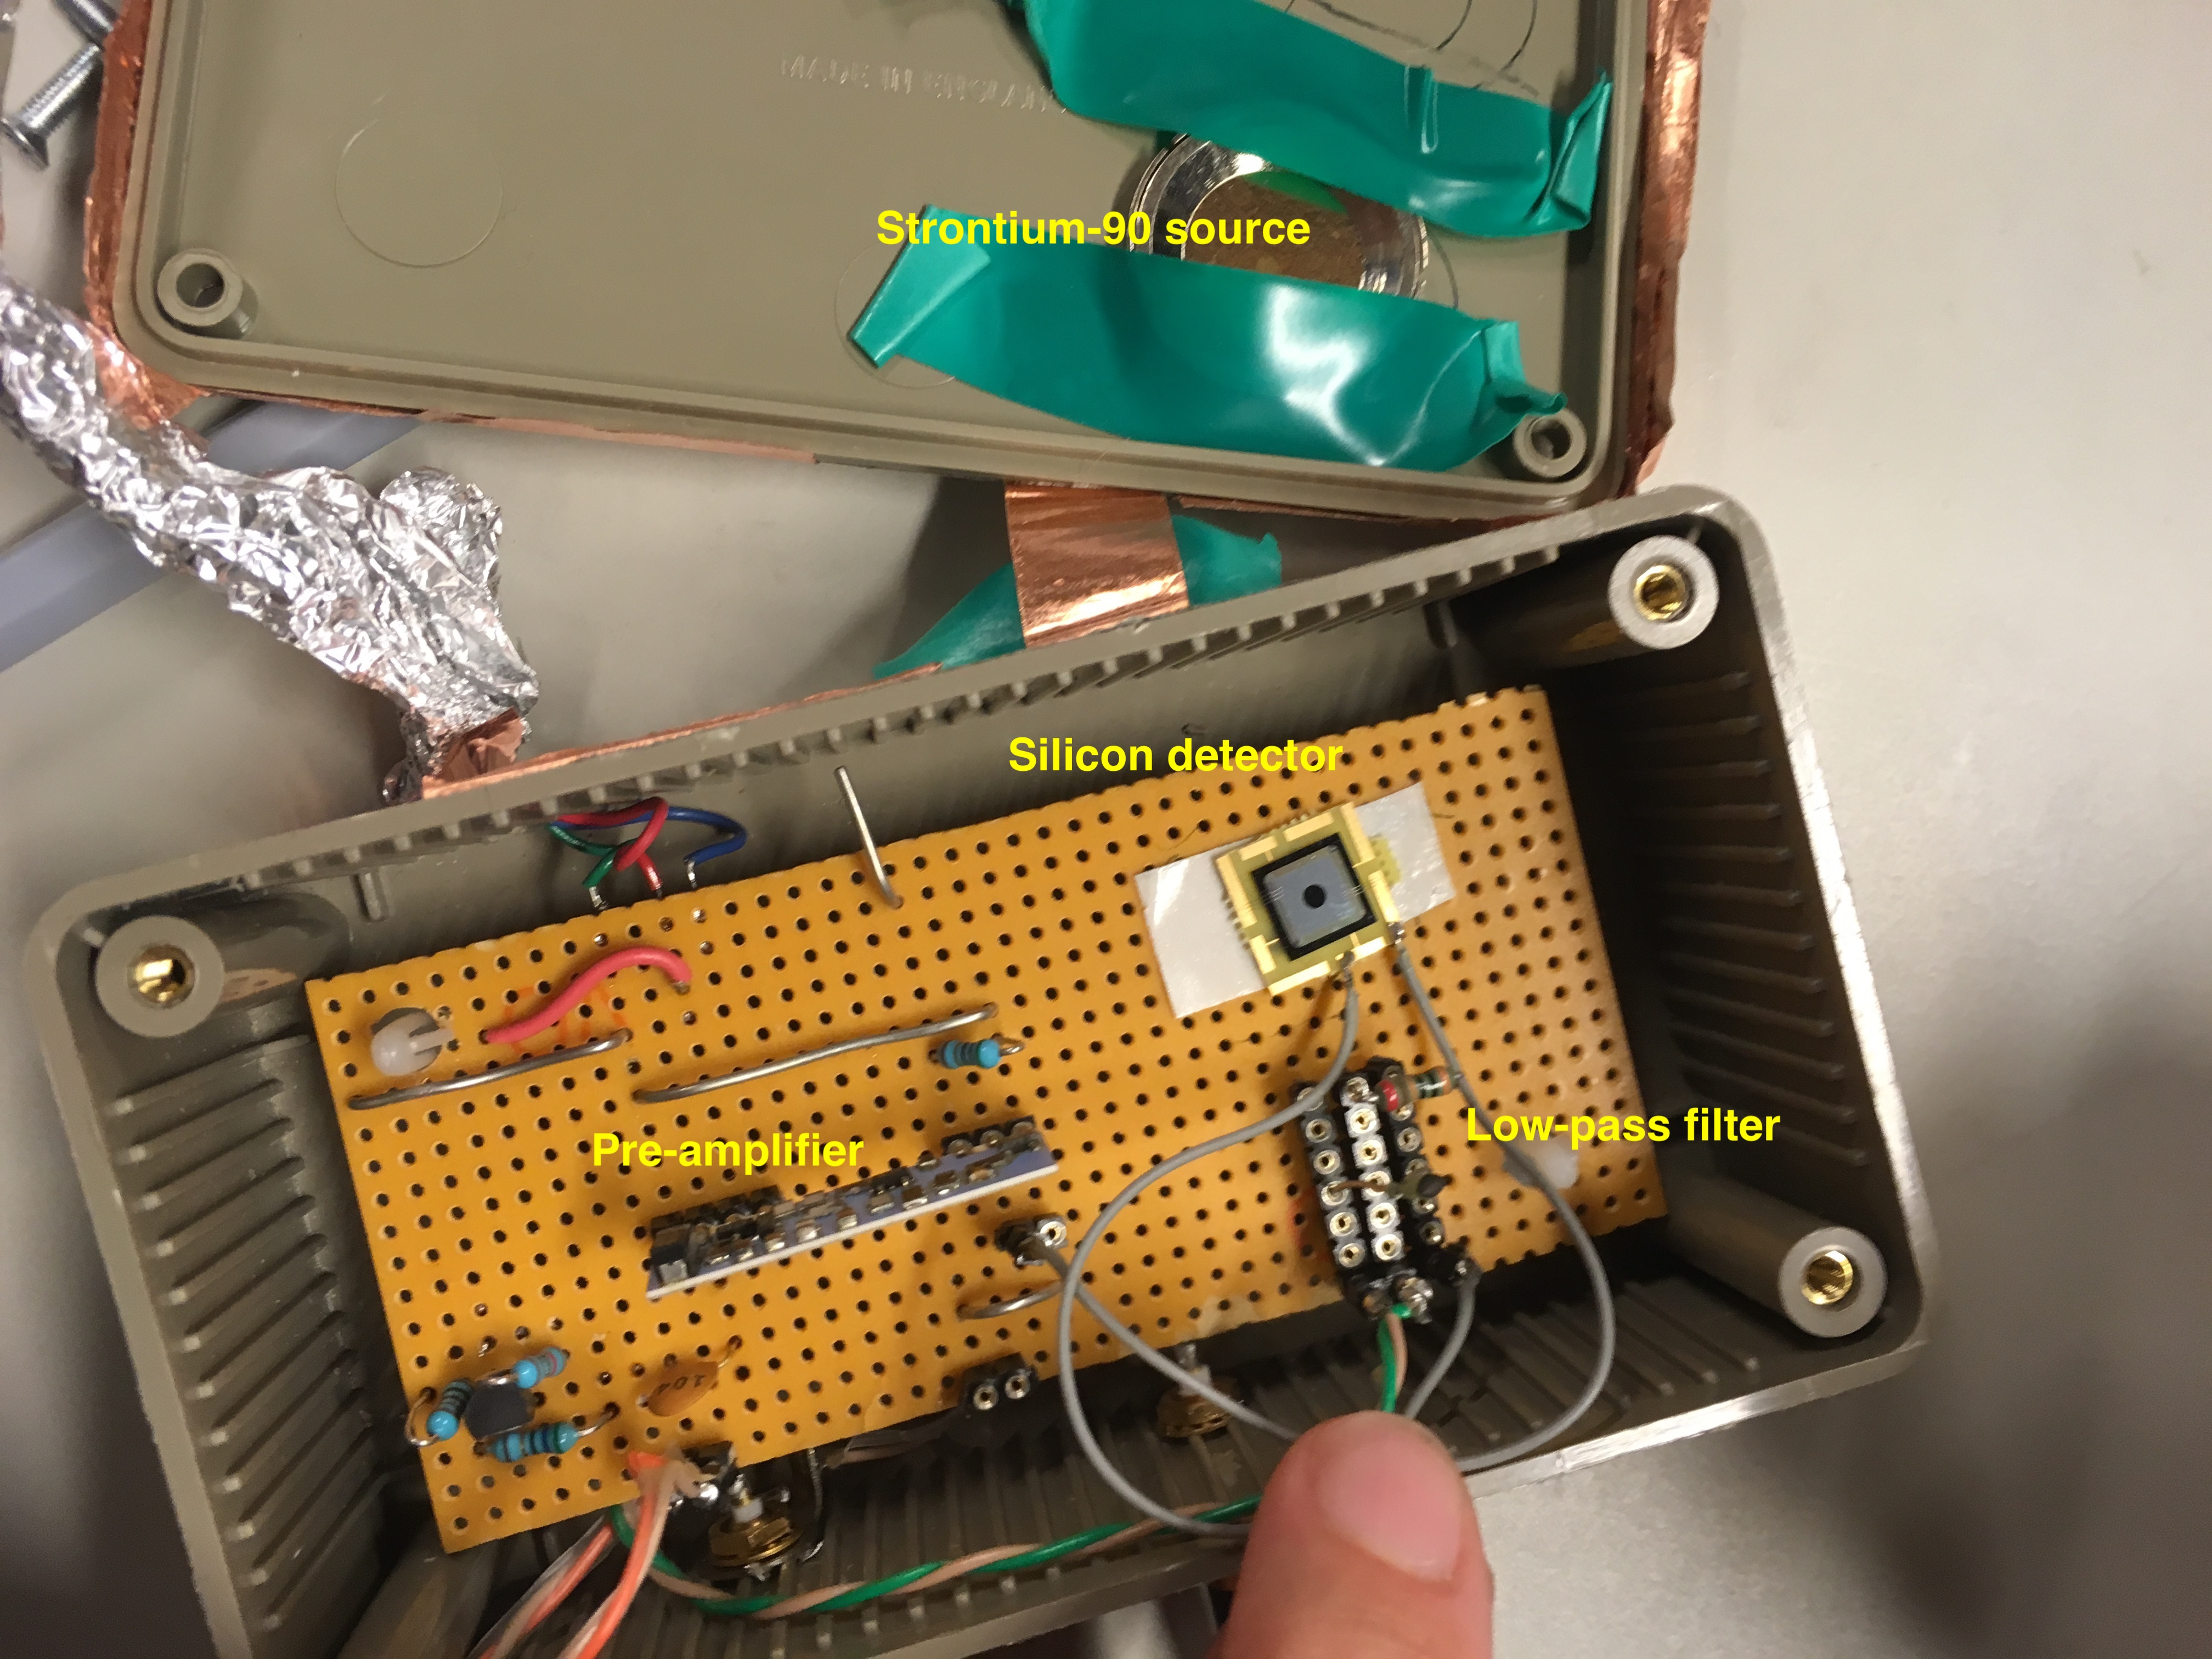
\includegraphics[width=0.8\textwidth]{./graphics/experimentalSetup}
  \caption{Silicon detector experimental setup.}
  \label{fig:ExperimentalSetpu}
\end{figure}

Before attaching the sensor to the rest of the circuit to perform measurements, the response of the pre-amplifier was calibrated using different capacitances between $1$ pF and $100$ pF put in parallel to the capacitance of $0.4$ pF at the calibration input. To do this, the amplifier was supplied with two voltage biases of + and -12V from a DC workbench power supply. The RMS of the baseline noise was measured while no pulse was injected. The circuit was fed with a square pulse and the rise time of the output signal was measured directly on the oscilloscope between the $10\%$ and $90\%$ of the rising signal. The amplitude of the signal was noted as well. During these measurements, the circuit and the cables were coated with aluminium foil (grounded through a cable to the HV power supply), in order to shield the system from radiations, which would cause additional noise to the output signal.

After the calibration measurements were completed, the silicon detector was introduced in the circuit by connecting it to the pre-amplifier. A voltage of around $60$ V was fed to the sensor, in order to fully deplete it, through a low-pass filter consisting of a $100$ nF capacitance and of a $300$ k$\Omega$ resistor, see Figure \ref{fig:ExperimentalSetup}. The resulting circuit is schematically shown in Figure \ref{fig:SiliconDiodeCircuit}.
Finally the Strontium-90 source was attached with tape to the lid of the box containig the entire circuit. By closing the lid and covering it with aliminium foil, external radiations were shielded. The measurement of the pulses induced in the silicon detector by the particles radiated by the Strontium decay were registered from the oscilloscoper for further analysis.

\begin{figure}[htb]
  \centering
  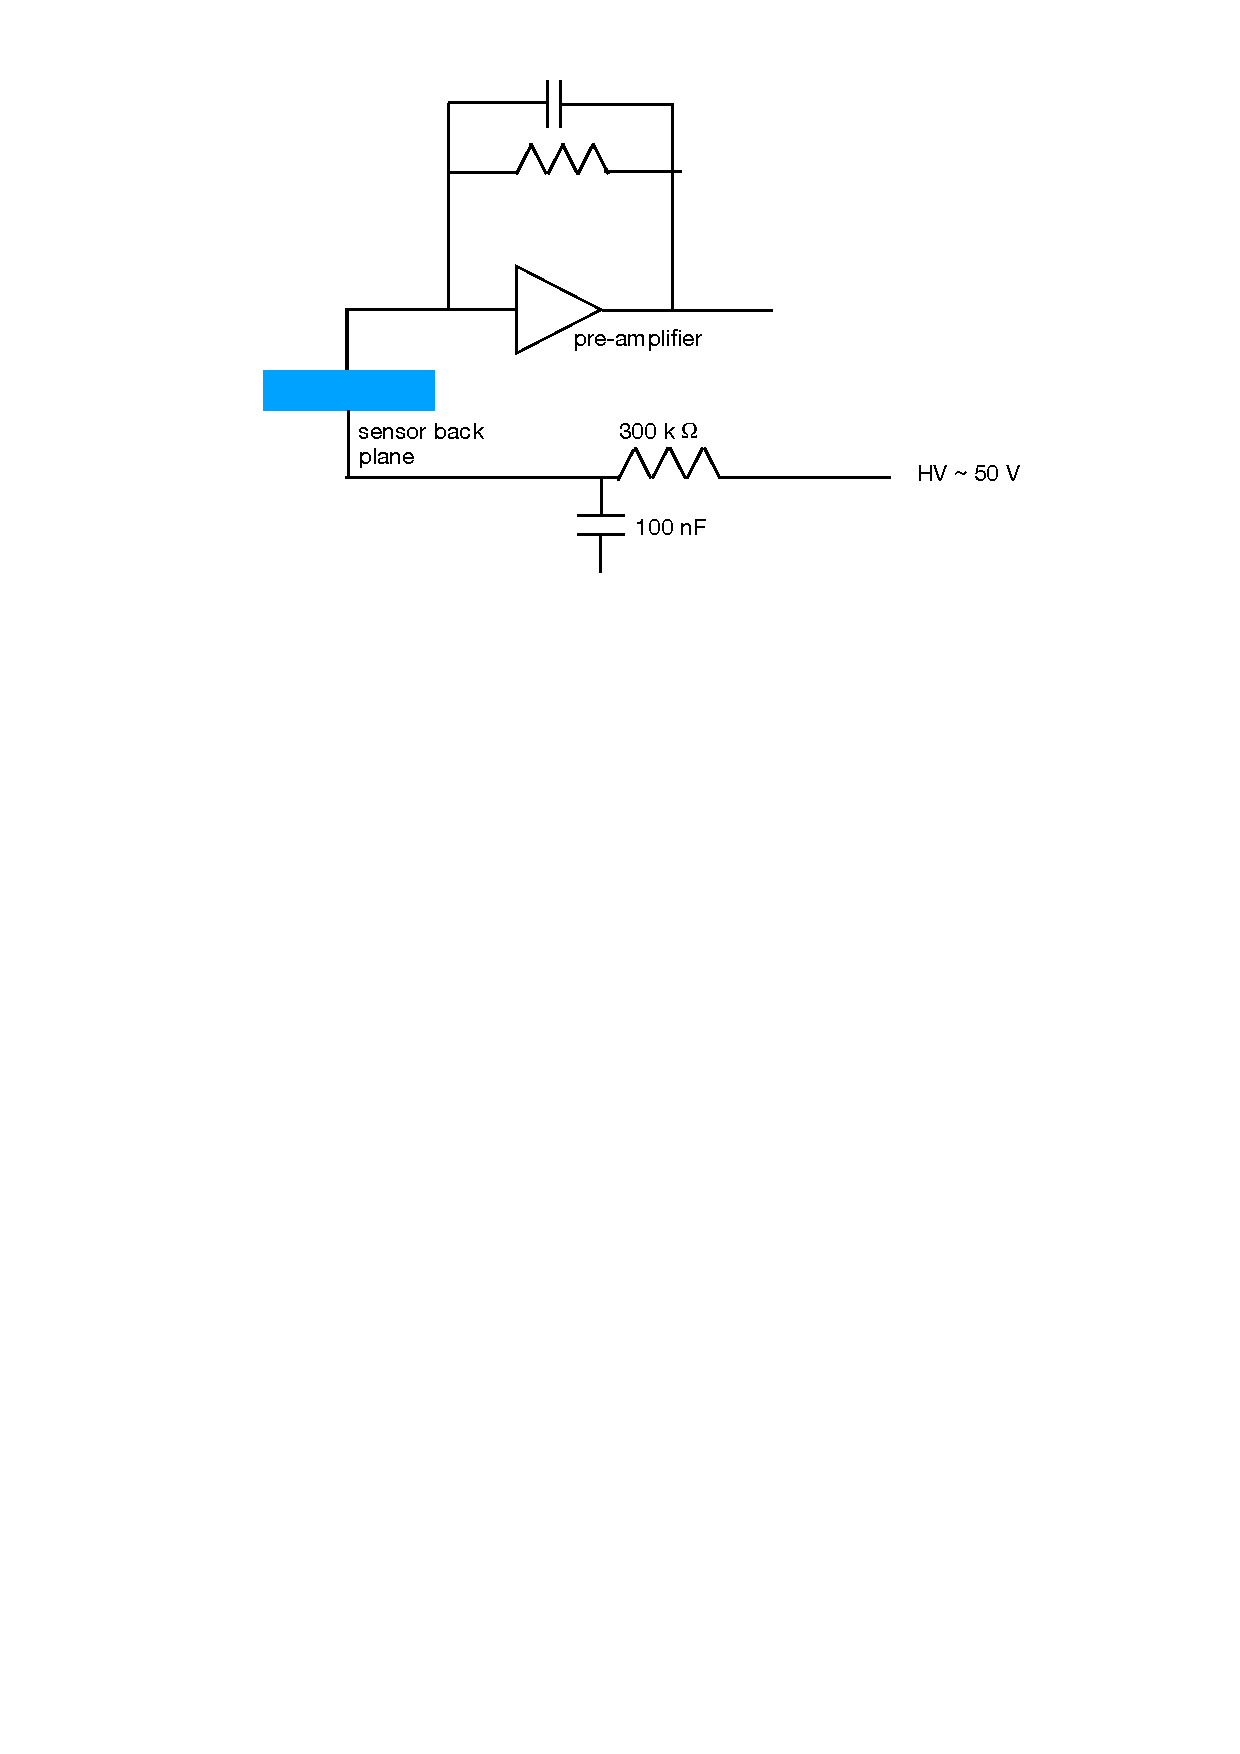
\includegraphics[width=0.8\textwidth]{./graphics/SiliconDiodeCircuit}
  \caption{Silicon detector circuit with low-pass filter, pre-amplifier and silicon diode.}
  \label{fig:SiliconDiodeCircuit}
\end{figure}

%More about the above: The wave supplies a fixed amount of electrons to the pre-amp. That amount can be converted from voltage to charge using the formula:

%\begin{equation}
%  Q = C\cdot V
%\end{equation}

%The capacitance $C$ is going to be the capacitance added to the circuit, in the case of the RMS noise. The charge of the output signal can also be converted into a charge value, but then the capacitance to use must be the sum of the Calib.in capacitance (0.4 pF) and the capacitance that is being added to the circuit.

%Amplitude of the result is 70 percent of the calibration amplitude due to different impedance matching.
%42mv became 32mV after termination (termination = channel at 50 Ohm impedance).

\section{Study of Silicon detector}

Before integrating the silicon detector inside the rest of the circuit, a few measurements were undertaken to undertand its properties: the depletion voltage and the capacitance at depletion. The IV curve measures the leakage current as a function of voltage and it is useful for measuring the deplation voltage. As it is visible from Figure \ref{fig:IVcurve}, the depletion voltage for this particular silicon diode is of $\approx 50$ V.

\begin{figure}[htb]
  \centering
  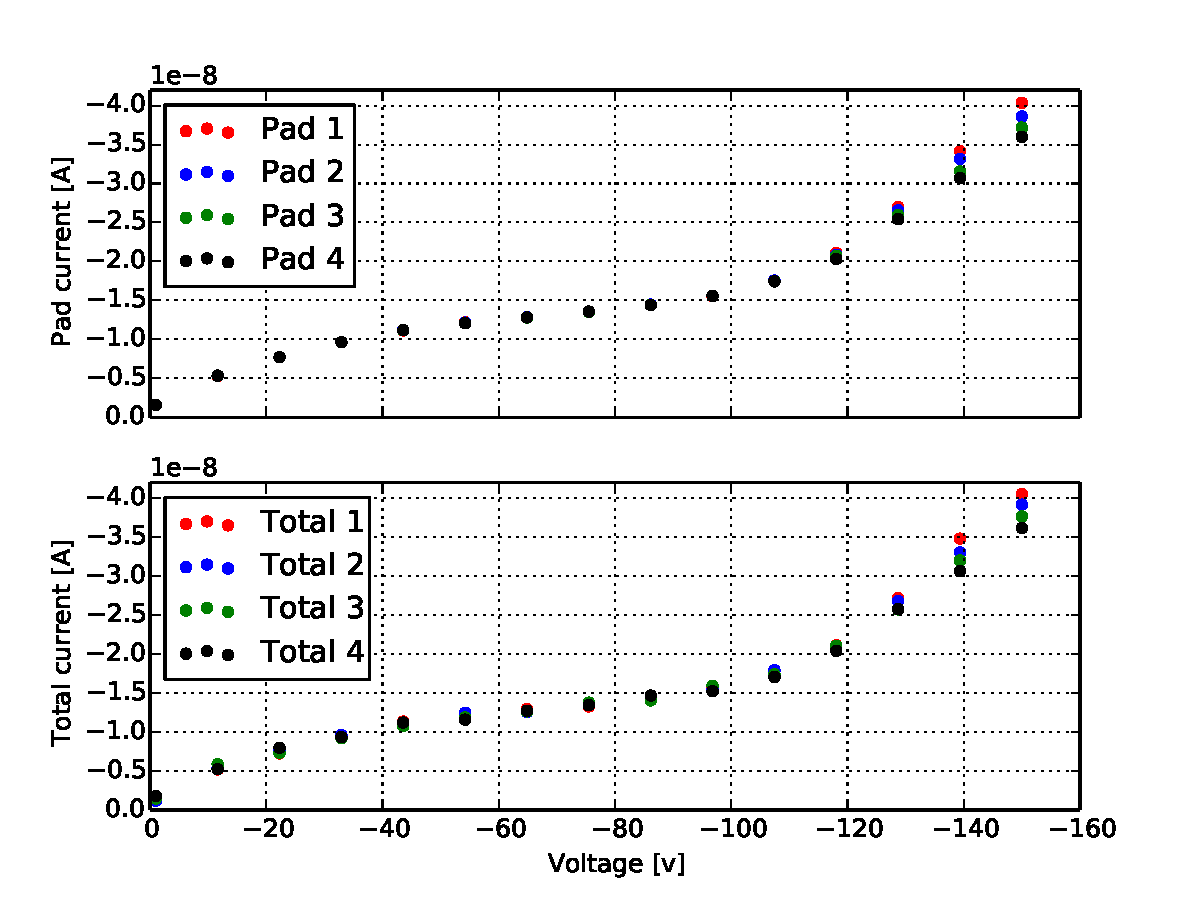
\includegraphics[width=0.8\textwidth]{./graphics/IV_V_vs_A.pdf}
  \caption{IV curve for the silicon detector of p-type. The upper plot shows the current per pad for the $4$ different pads, while the lower plot shows the total current }
  \label{fig:IVcurve}
\end{figure}

\begin{figure}[t!]
  \centering
  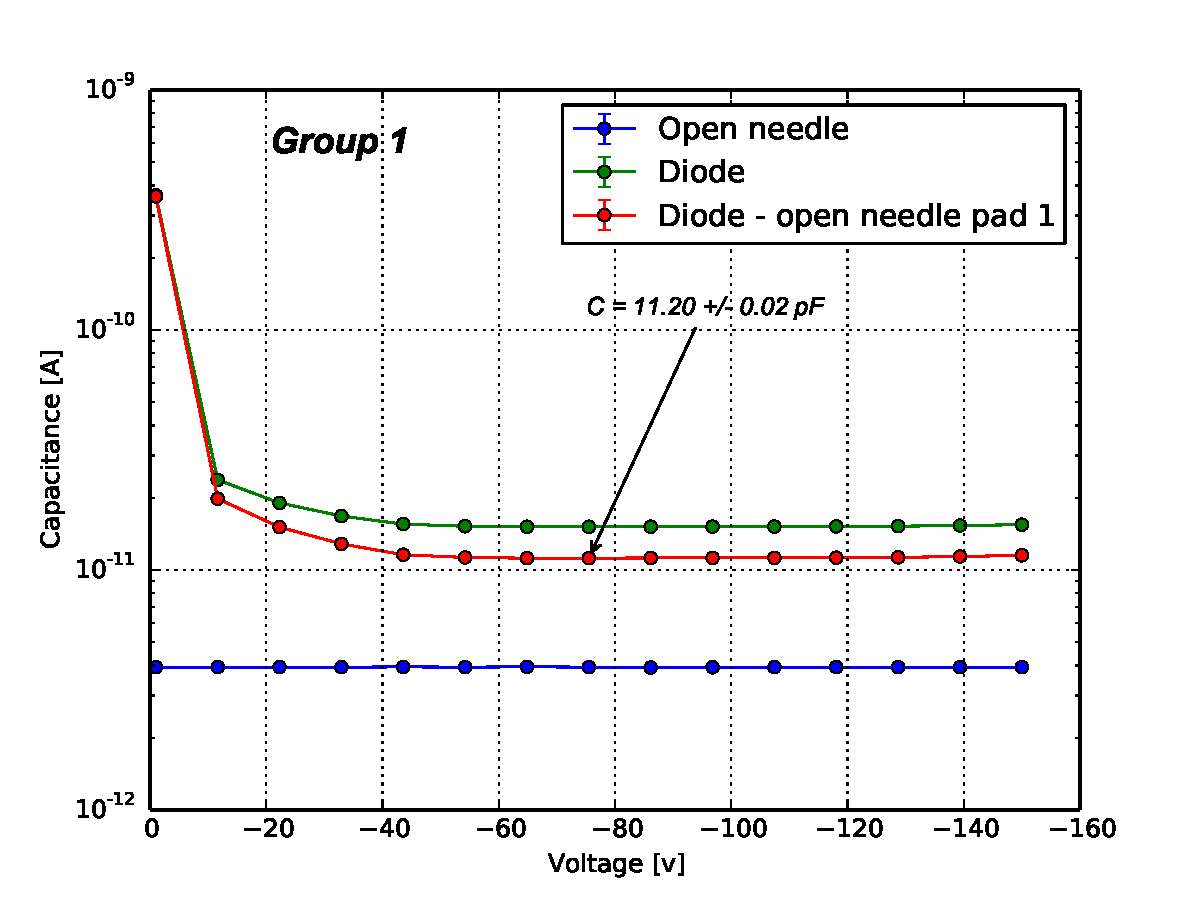
\includegraphics[width=1.2\textwidth]{./graphics/V_vs_C}
  \caption{Parasitic capacitance of the instrument (blue), capacitance of the system plus the silicon diode and capacitance of the diode as a function of voltage.}
  \label{fig:VC_curve_single}
\end{figure}

\section{Pre-amplifier calibration}

\begin{figure}[htb]
  \centering
  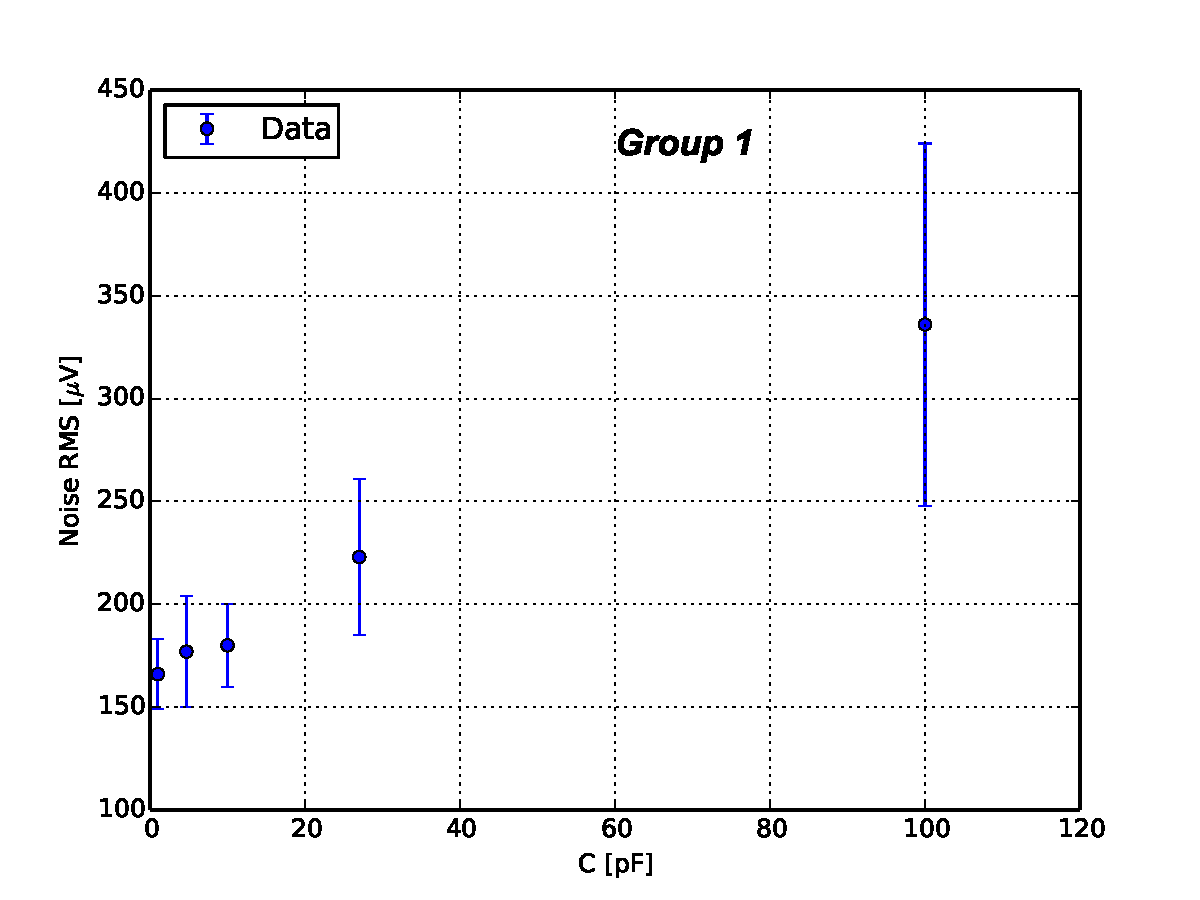
\includegraphics[width=0.8\textwidth]{./graphics/noise_vs_capacitance}
  \caption{Noise RMS vs capacitance measurement}
  \label{fig:Noise_vs_Capacitance}
\end{figure}

\begin{figure}[htb]
  \centering
  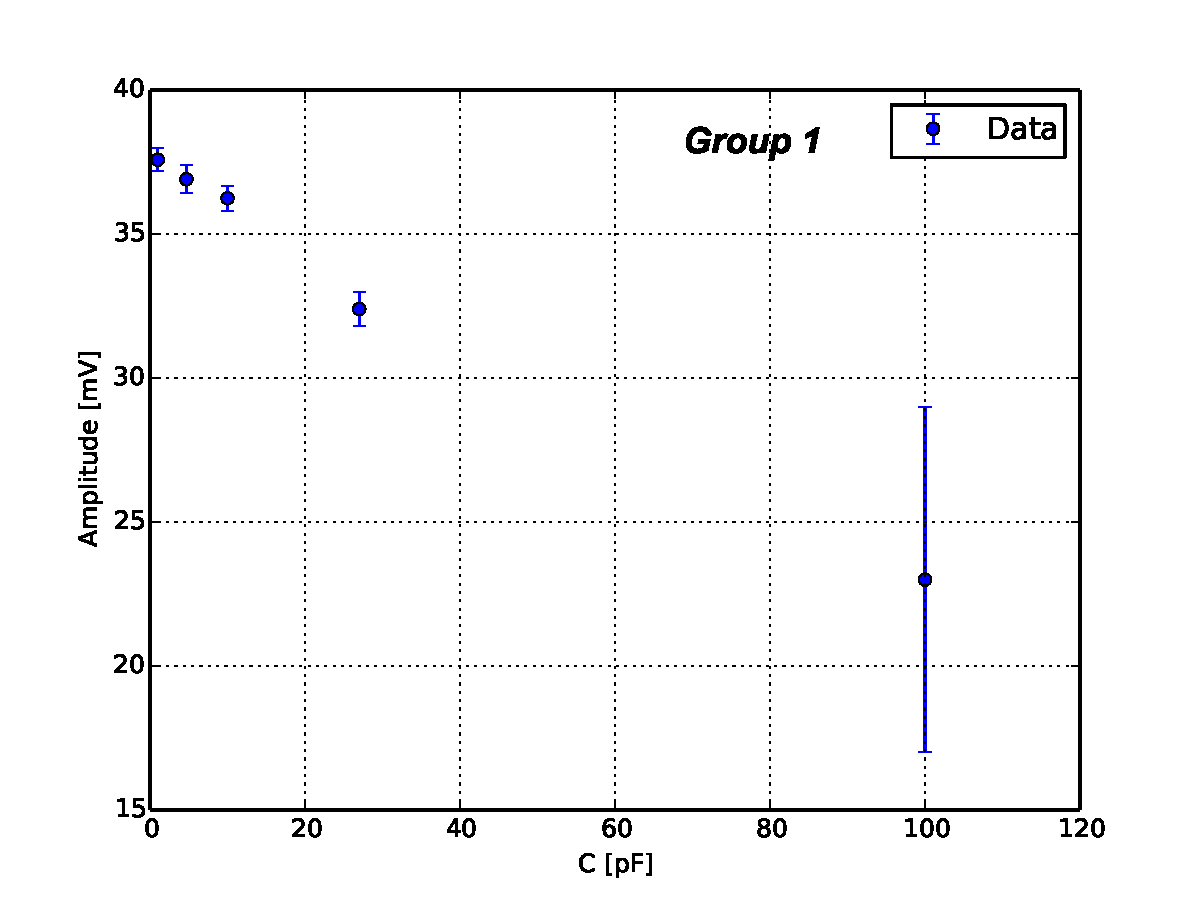
\includegraphics[width=0.8\textwidth]{./graphics/amplitude_vs_capacitance}
  \caption{Amplitude vs capacitance measurement}
  \label{fig:Amplitude_vs_Capacitance}
\end{figure}

% This figure should be for the ENC curve - when I figure out how to calculate it
%\begin{figure}[htb]
%  \centering
%  \includegraphics[width=0.8\textwidth]{./graphics/}
%  \caption{}
%  \label{fig:}
%\end{figure}

\begin{figure}[htb]
  \centering
  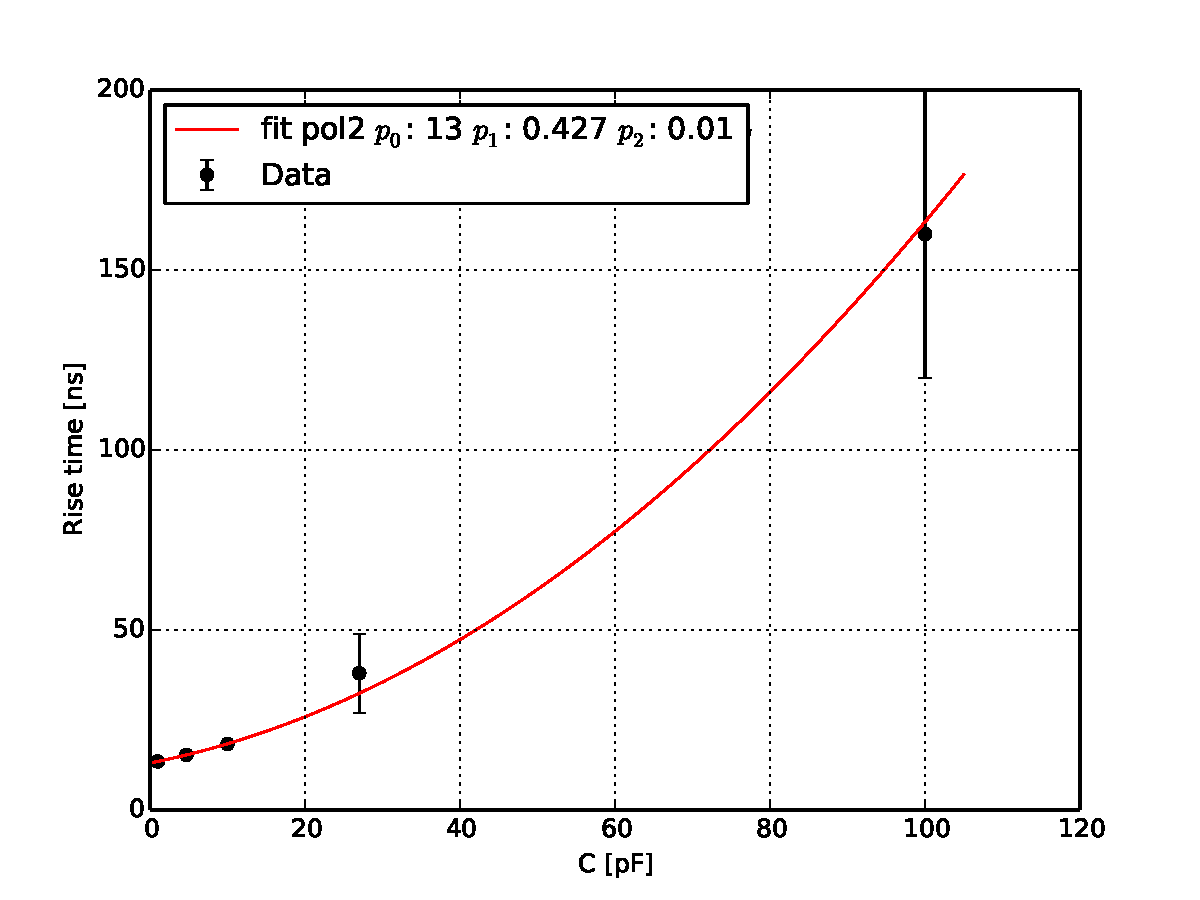
\includegraphics[width=0.8\textwidth]{./graphics/calibration_diode}
  \caption{Calibration of the rise time as a function of capacitance}
  \label{fig:RiseTime_vs_Capacitance}
\end{figure}

\section{Results}

\begin{figure}[t!]
  \centering
  \begin{subfigure}[t]{0.45\textwidth}
    \centering
    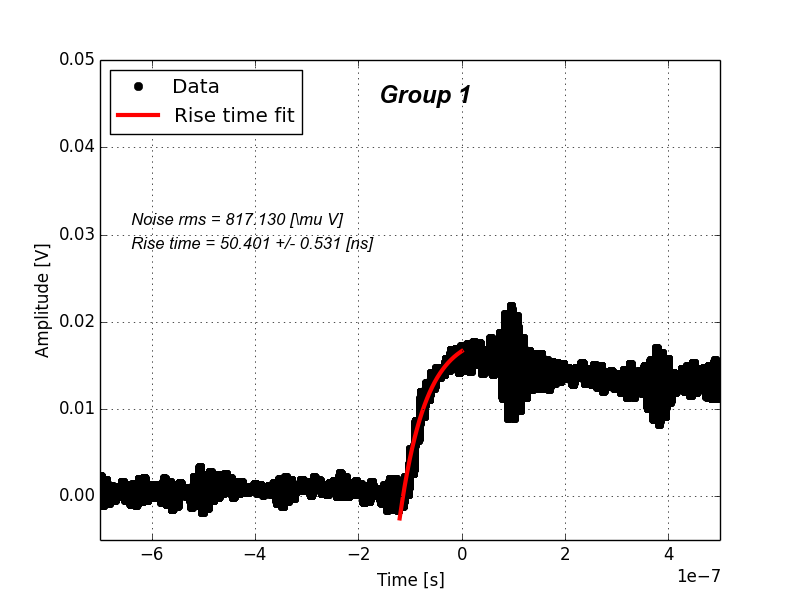
\includegraphics[width=1.2\textwidth]{./graphics/data_0.png}
  \end{subfigure}
  \hfill
  \begin{subfigure}[t]{0.45\textwidth}
    \centering
    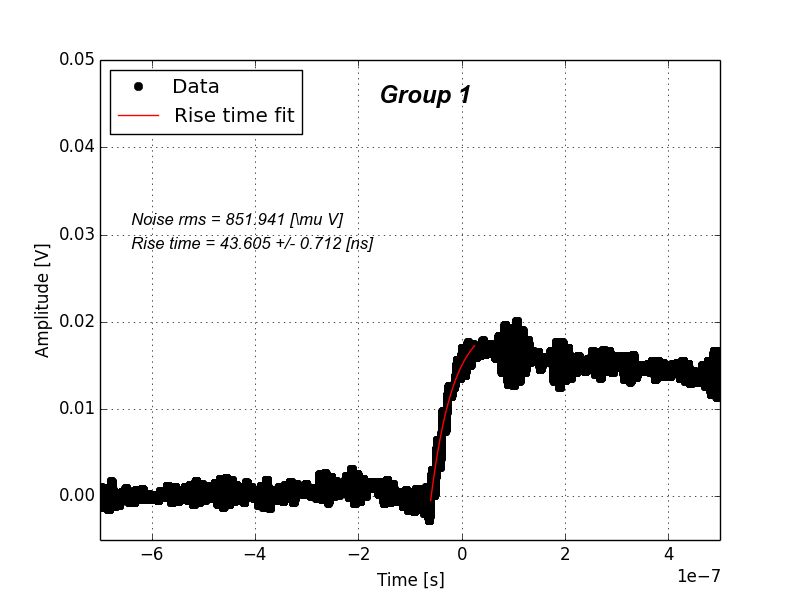
\includegraphics[width=1.2\textwidth]{./graphics/data_1.png}
  \end{subfigure}
  \hfill
  \begin{subfigure}[t]{0.45\textwidth}
    \centering
    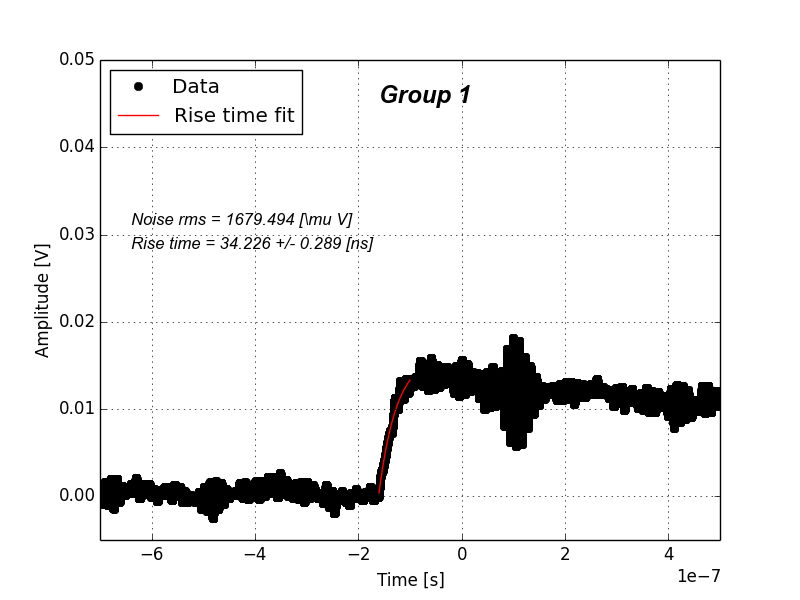
\includegraphics[width=1.2\textwidth]{./graphics/data_2.png}
  \end{subfigure}
  \hfill
  \begin{subfigure}[t]{0.45\textwidth}
    \centering
    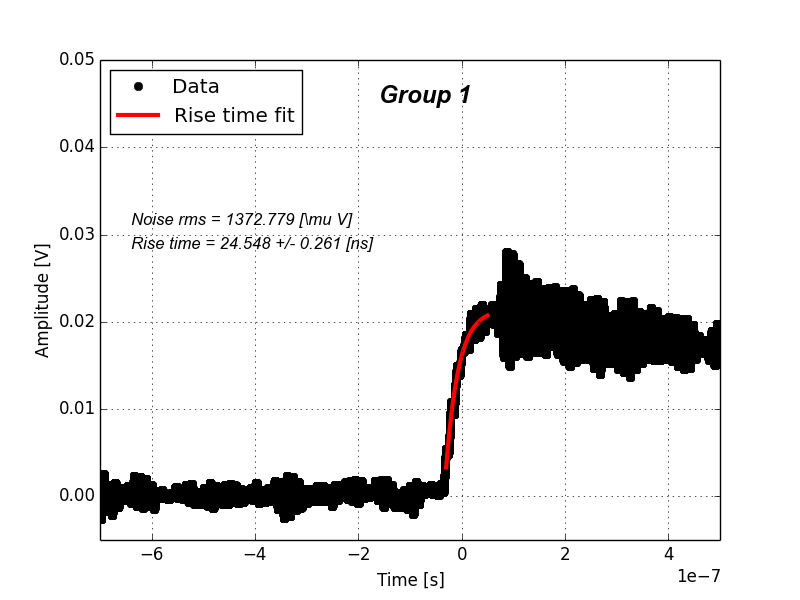
\includegraphics[width=1.2\textwidth]{./graphics/data_3.png}
  \end{subfigure}
  \hfill
  \begin{subfigure}[t]{0.45\textwidth}
    \centering
    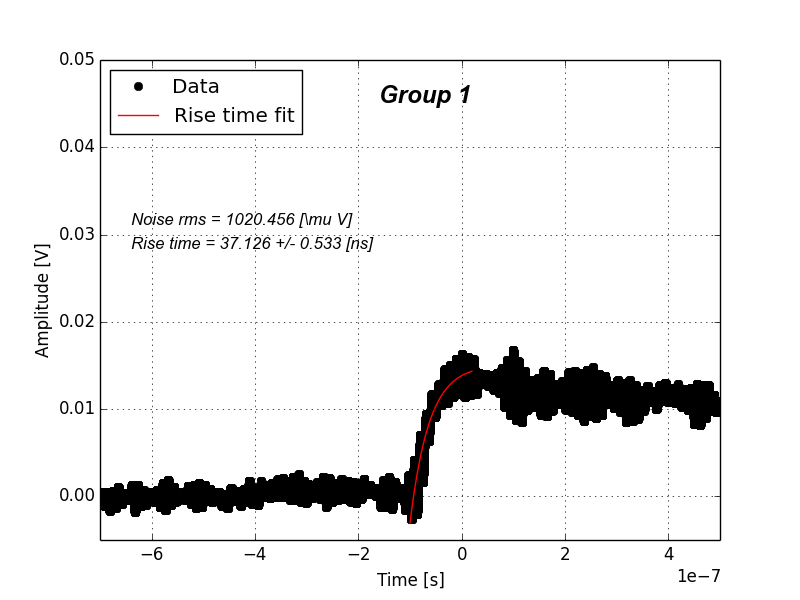
\includegraphics[width=1.2\textwidth]{./graphics/data_4.png}
  \end{subfigure}
  \hfill
  \begin{subfigure}[t]{0.45\textwidth}
    \centering
    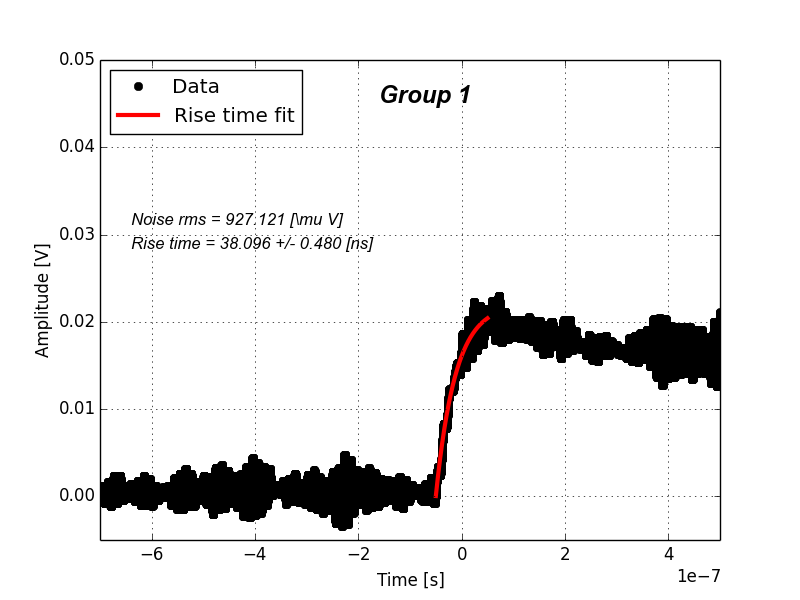
\includegraphics[width=1.2\textwidth]{./graphics/data_5.png}
  \end{subfigure}
\caption{Measurement of the rise time from the Strontium-90 decay}
\label{fig:rise_time_measurement}
\end{figure}
\begin{figure}[t!]
  \centering
  \begin{subfigure}[t]{0.45\textwidth}
    \centering
    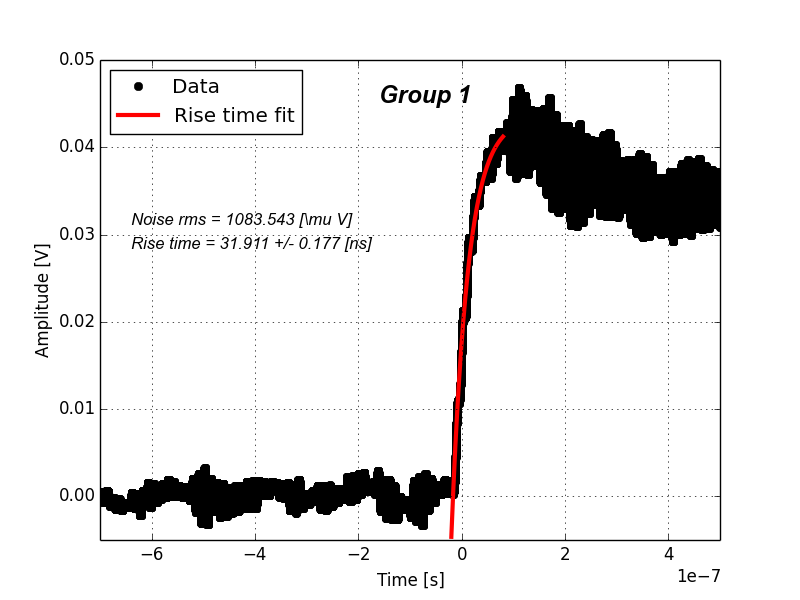
\includegraphics[width=1.2\textwidth]{./graphics/data_6.png}
  \end{subfigure}
  \hfill
  \begin{subfigure}[t]{0.45\textwidth}
    \centering
    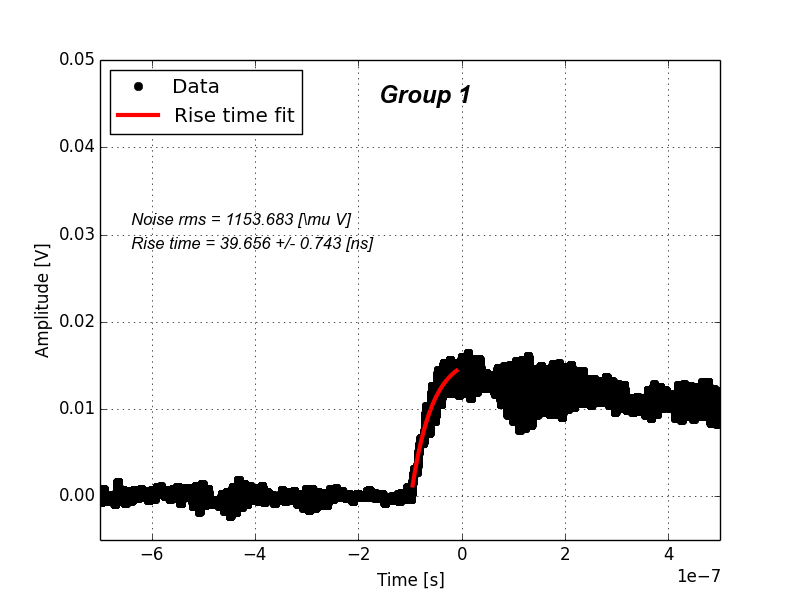
\includegraphics[width=1.2\textwidth]{./graphics/data_7.png}
  \end{subfigure}
  \hfill
  \begin{subfigure}[t]{0.45\textwidth}
    \centering
    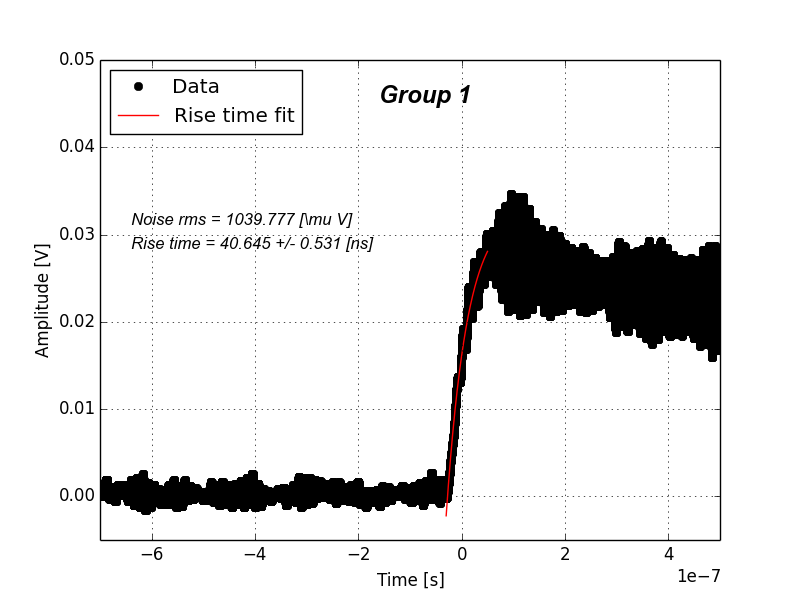
\includegraphics[width=1.2\textwidth]{./graphics/data_8.png}
  \end{subfigure}
  \hfill
  \begin{subfigure}[t]{0.45\textwidth}
    \centering
    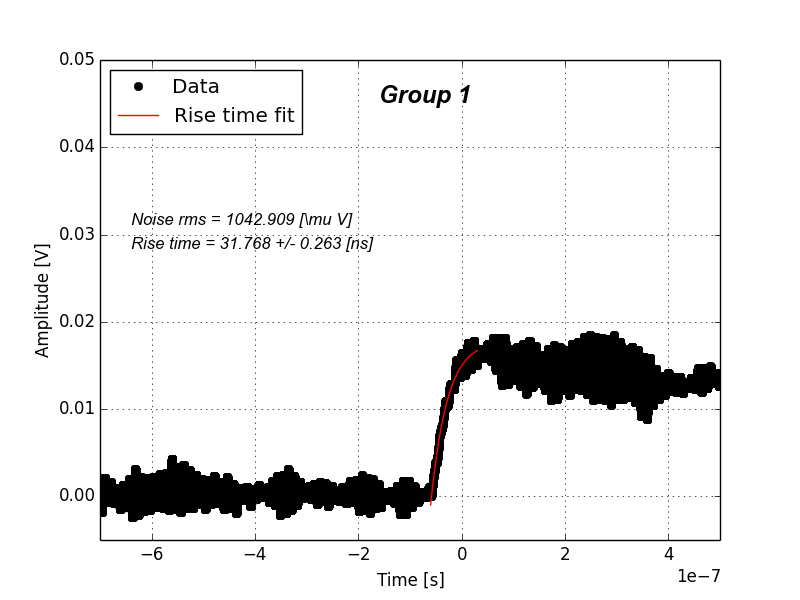
\includegraphics[width=1.2\textwidth]{./graphics/data_9.png}
  \end{subfigure}
  \hfill
  \begin{subfigure}[t]{0.45\textwidth}
    \centering
    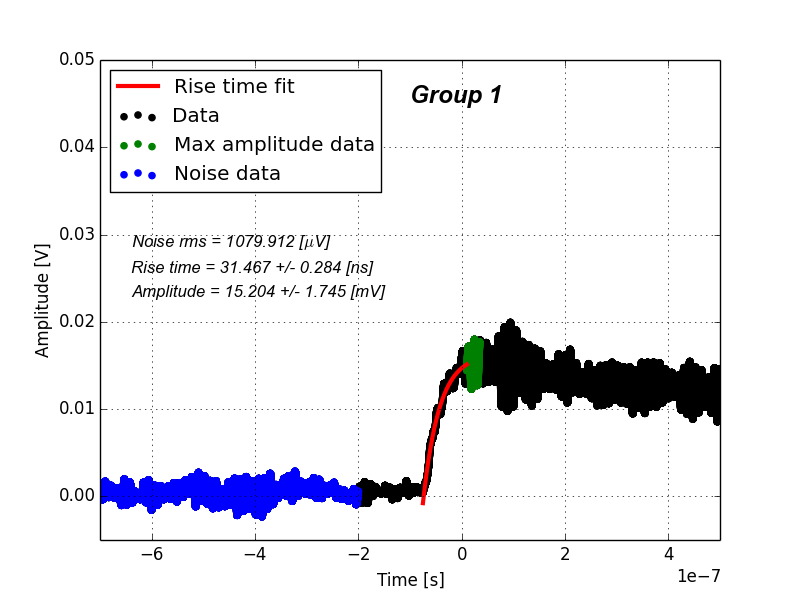
\includegraphics[width=1.2\textwidth]{./graphics/data_10.png}
  \end{subfigure}
  \hfill
  \begin{subfigure}[t]{0.45\textwidth}
    \centering
    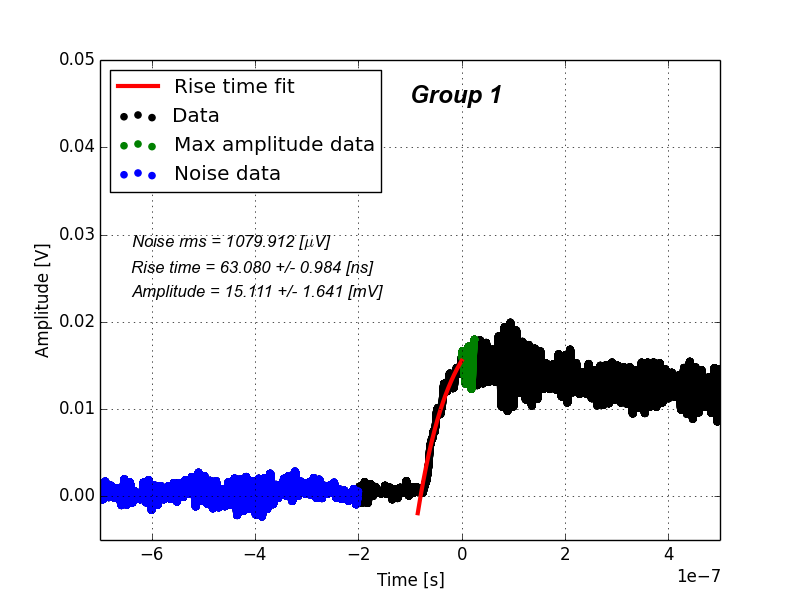
\includegraphics[width=1.2\textwidth]{./graphics/data_11.png}
  \end{subfigure}
\caption{Measurement of the rise time from the Strontium-90 decay}
\label{fig:rise_time_measurement}
\end{figure}

\begin{figure}[htb]
  \centering
  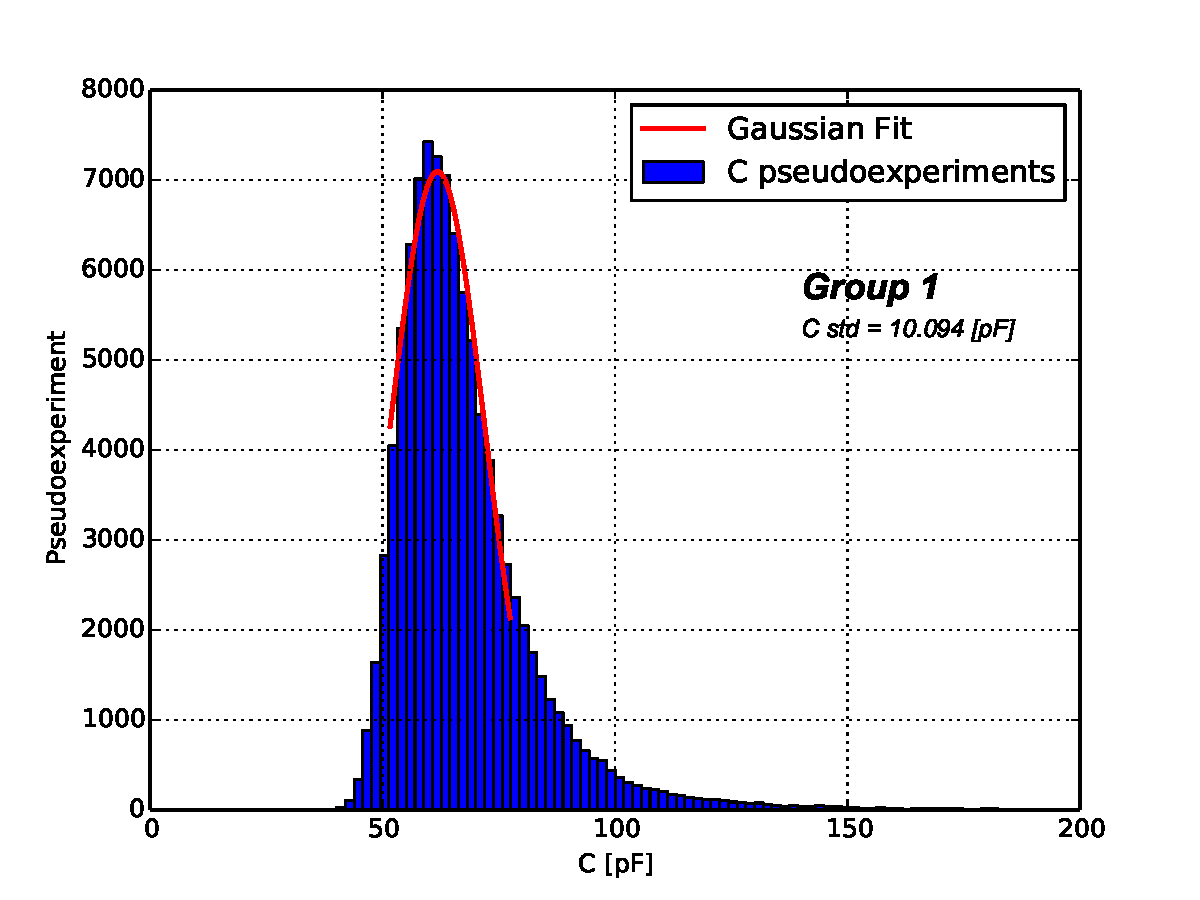
\includegraphics[width=0.8\textwidth]{./graphics/stat_error_on_C_pseudoexperiments}
  \caption{Statistical error on C from MC pseudoexperiments}
  \label{fig:stat_error_on_C}
\end{figure}

\section{Discussion}
\section{Conclusion}




















\end{document}
